\documentclass{standalone}
\usepackage{tikz}
\usepackage{xcolor}
\usepackage{ifthen}
\usepackage{amsmath, amssymb}

\begin{document}

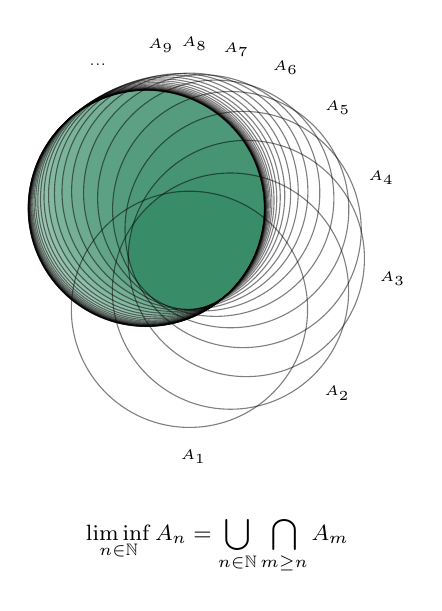
\begin{tikzpicture}[scale=1.5]

    % Define colors
    \definecolor{lightgreen}{RGB}{34, 139, 34}
    \definecolor{calpolypomonagreen}{rgb}{0.12, 0.3, 0.17}
    \definecolor{cadmiumgreen}{rgb}{0.0, 0.42, 0.24}

    % Set the distance of the circle centers from the origin
    \def\distance{0.5}

    % Set the radius of the circles
    \def\radius{1}

    % Define the angle range
    \def\startAngle{135}
    \def\endAngle{-135}
    \def\n{30} % Number of circles
    
    % Compute the angular step between circles
    \pgfmathsetmacro{\angleStep}{(\startAngle - \endAngle)/(\n-1)}


    \foreach \m in {1, ...,\n} {
        % Shade the intersection of all circles
        \begin{scope}
            % Start clipping with the first circle
            \pgfmathsetmacro{\currentAngle}{\startAngle}
            \pgfmathsetmacro{\xCenter}{\distance * cos(\currentAngle)}
            \pgfmathsetmacro{\yCenter}{\distance * sin(\currentAngle)}
            \clip (\xCenter, \yCenter) circle (\radius);
            
            % Clip with the remaining circles
            \foreach \i in {\m,...,\n} {
                \pgfmathsetmacro{\currentAngle}{\startAngle - (4/5)^\i*\n * \angleStep}
                \pgfmathsetmacro{\xCenter}{\distance * cos(\currentAngle)}
                \pgfmathsetmacro{\yCenter}{\distance * sin(\currentAngle)}
                
                \clip (\xCenter, \yCenter) circle (\radius); % Clip with each subsequent circle
            }
            % Fill the common intersection area with a color
            \fill[lightgreen, fill opacity = (\n-\m)/\n*0.1, color = cadmiumgreen] (-3, -3) rectangle (3, 3); % Large enough to cover the intersection area
        \end{scope}
    }

    % Draw the n circles from 135º to -135º
    \foreach \i in {1,...,\n} {
        \pgfmathsetmacro{\currentAngle}{\startAngle - (4/5)^\i*\n * \angleStep}
        \pgfmathsetmacro{\xCenter}{\distance * cos(\currentAngle)}
        \pgfmathsetmacro{\yCenter}{\distance * sin(\currentAngle)}
        
        % Draw each circle with the given radius
        \draw [opacity=0.5] (\xCenter, \yCenter) circle (\radius);
        \ifthenelse{\i<10}{
        \pgfmathsetmacro{\xLabel}{1.75 * cos(\currentAngle)};
        \pgfmathsetmacro{\yLabel}{1.75 * sin(\currentAngle)};
        \node at (\xLabel, \yLabel) {\tiny $A_{\i}$};
        }{
            \ifthenelse{\i=12}{
            \pgfmathsetmacro{\xLabel}{1.75 * cos(\currentAngle)};
            \pgfmathsetmacro{\yLabel}{1.75 * sin(\currentAngle)};
            \node at (\xLabel, \yLabel) {\tiny ...};
            }{}
        }
    }

    \node at (0.25,-2.5) {\footnotesize $\displaystyle\liminf_{n \in \mathbb N} A_n = \bigcup_{n \in \mathbb N} \bigcap_{m \geq n} A_m $};

\end{tikzpicture}

\end{document}
